\documentclass[a4paper, 12pt]{article}

\def\languages{french, english}

%%%%%%%%%%%%%%%%%%% Libraries

%%%%%%%%%% Packages

%%%%% Coding tools

\usepackage{comment}
\usepackage{xstring}

%%%%% Encoding

\usepackage[utf8]{inputenc}
\usepackage[T1]{fontenc}
\usepackage{eurosym}

%%%%% Languages

\ifx\languages\undefined
	\usepackage[english]{babel}
\else
	\usepackage[\languages]{babel}
\fi

\def\languagefile{./include/languages/\languagename.tex}
\InputIfFileExists{\languagefile}{}

%%%%% Style

\usepackage{geometry}
\usepackage{fancyhdr}
\usepackage[bottom]{footmisc}

\edef\restoreparindent{\parindent=\the\parindent\relax}
\usepackage[parfill]{parskip}

\usepackage{enumitem}
\usepackage{csquotes}
\usepackage{color}

%%%%% Others

\usepackage[framemethod=TikZ]{mdframed}
\usepackage[pdfusetitle]{hyperref}

%%%%%%%%%% Features

%%%%% Settings

\geometry{paper=a4paper,top=3.5cm,bottom=2.5cm,right=2.5cm,left=2.5cm}

\pagestyle{fancy}
\fancyhead[L]{}
\fancyhead[R]{\leftmark}
\fancyfoot[C]{\thepage}
\renewcommand{\headrulewidth}{0pt}

%\restoreparindent

%%%%% Commands

\newcommand{\romantableofcontents}{
	\newpage
	\pagenumbering{roman}
	\tableofcontents
	\newpage
	\pagenumbering{arabic}
}

%%%%%%%%%% Packages

\usepackage{float}
\usepackage[skip=1em]{caption}
\usepackage{subcaption}

\usepackage{array}
\usepackage{multirow}
\usepackage{multicol}

%%%%%%%%%% Features

%%%%% Settings

\renewcommand{\arraystretch}{1.2}

%%%%% Commands

\newcommand\noskipcaption[1]{\caption{#1}\vspace{-1em}}
\newcommand\noskipcaptionstar[1]{\caption*{#1}\vspace{-1em}}

%%%%%%%%%% Packages

\usepackage{amsmath}
\usepackage{amssymb}
\usepackage{bm}
\usepackage{esint}
\usepackage[makeroom]{cancel}

%%%%%%%%%% Features

%%%%% Macros

\newcommand{\rbk}[1]{\left(#1\right)}
\newcommand{\cbk}[1]{\left\{#1\right\}}
\newcommand{\sbk}[1]{\left[#1\right]}
\newcommand{\abs}[1]{\left|#1\right|}
\newcommand{\norm}[1]{\left\|#1\right\|}

\newcommand{\fact}[1]{#1!}
\newcommand{\e}[1]{\mathbf{e}_{#1}}
\newcommand{\deriv}{\mathrm{d}}
\DeclareMathOperator{\tr}{tr}

\def\Rl{\mathbb{R}}
\def\Cx{\mathbb{C}}
\def\Na{\mathbb{N}}
\def\Zi{\mathbb{Z}}

%%%%%%%%%% Packages

\usepackage{siunitx}

%%%%%%%%%% Features

%%%%% Settings

\ifx\decimalsign\undefined
\else
    \sisetup{output-decimal-marker = \decimalsign}
\fi


%%%%%%%%%%%%%%%%%%% Titlepage

\title{\vspace{-2cm}\textsc{ELEN0062} - Introduction to machine learning\\Project 1 - Classification algorithms}
\author{
François \textsc{Rozet} (s161024)\\
Adrien \textsc{Schoffeniels} (s162843)\\
}
\date{\today}

%%%%%%%%%%%%%%%%%%%

\newcommand{\X}{\mathcal{X}}
\newcommand{\Y}{\mathcal{Y}}
\newcommand{\Z}{\mathcal{Z}}

\DeclareMathOperator{\argmax}{argmax}
\DeclareMathOperator{\cor}{Cor}

%%%%%%%%%%%%%%%%%%%

\begin{document}
	\maketitle
	\section{Decision tree}
	\subsection{Decision boundary}
    \begin{enumerate}[label = (\alph*)]
        \item For both datasets (\texttt{make\_data1} and \texttt{make\_data2}) and for each maximum depth (\texttt{max\_depth}) value, a decision boundary graph\footnotemark{} has been produced using the \texttt{plot\_boundary} function, yielding Figures \ref{fig:decision_boundary_decision_tree_make_data1} and \ref{fig:decision_boundary_decision_tree_make_data2}.
        
        \footnotetext{For the sake of compactness, the decision boundary plots won't all be displayed. Moreover, in order to keep the boundaries visible, it has been chosen to display only the \num{150} first objects from the testing set.}
        
        \begin{figure}[h]
            \centering
            \begin{subfigure}{0.49\textwidth}
                \centering
        	    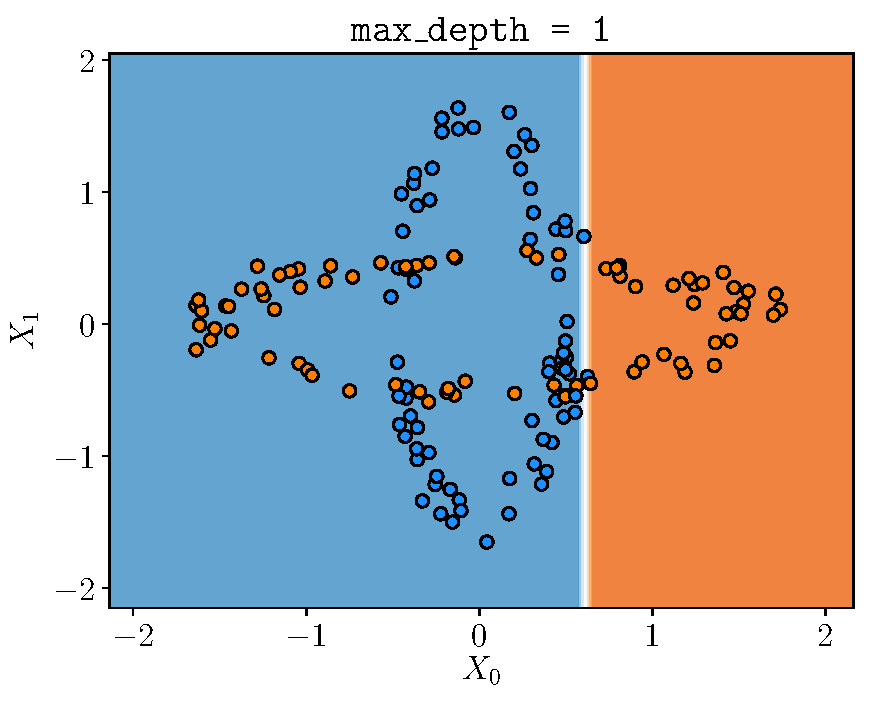
\includegraphics[width=0.85\textwidth]{resources/pdf/make_data1_depth1.pdf}
            \end{subfigure}
            \begin{subfigure}{0.49\textwidth}
                \centering
        	    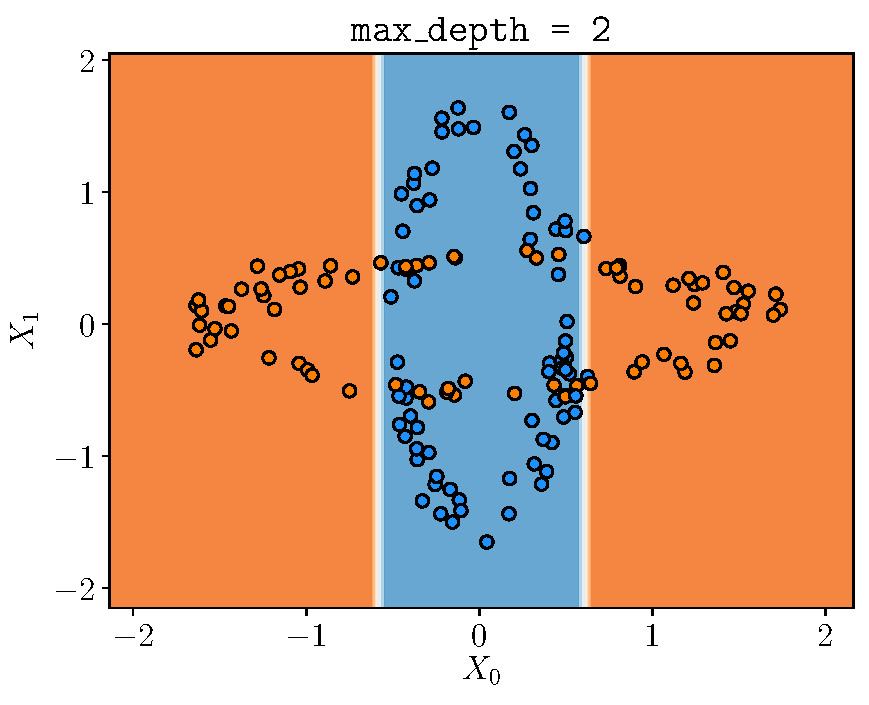
\includegraphics[width=0.85\textwidth]{resources/pdf/make_data1_depth2.pdf}
            \end{subfigure}
            \begin{subfigure}{0.49\textwidth}
                \centering
        	    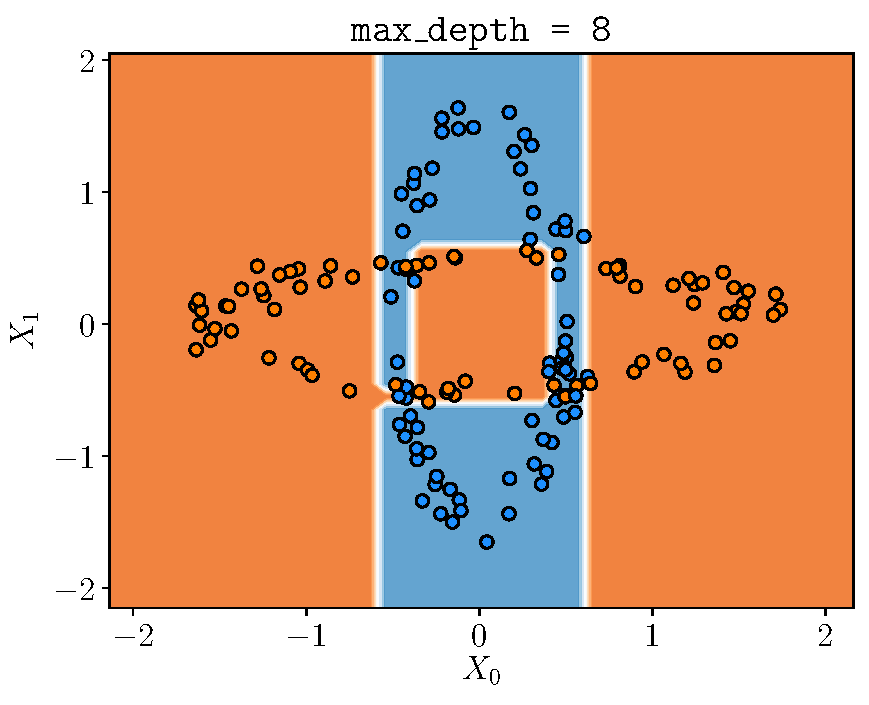
\includegraphics[width=0.85\textwidth]{resources/pdf/make_data1_depth8.pdf}
            \end{subfigure}
            \begin{subfigure}{0.49\textwidth}
                \centering
        	    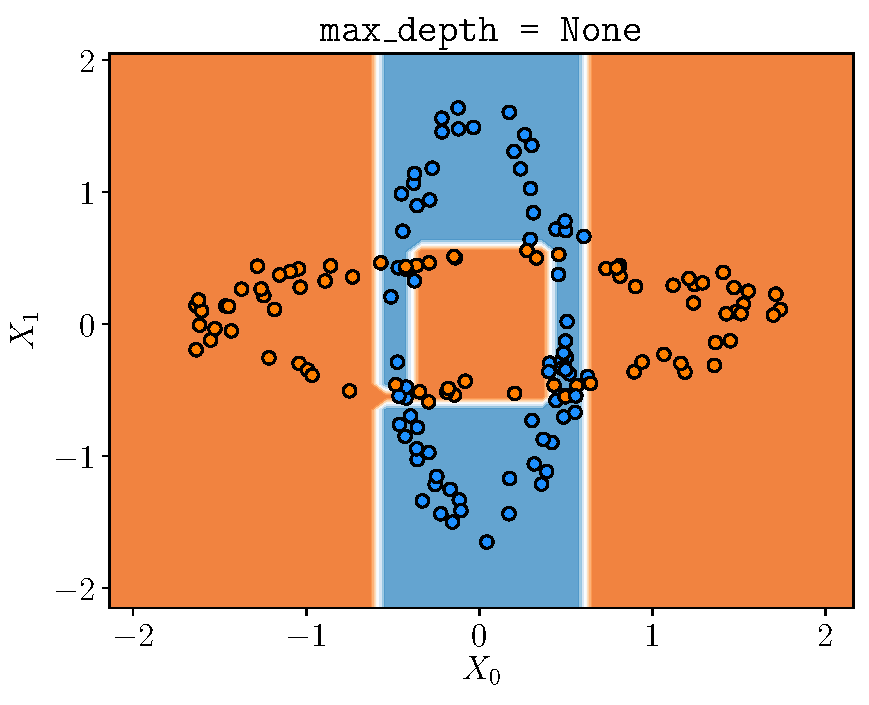
\includegraphics[width=0.85\textwidth]{resources/pdf/make_data1_depthNone.pdf}
            \end{subfigure}
            \noskipcaption{Decision boundary plots of decision tree models with fixed \texttt{max\_depth} for dataset \texttt{make\_data1}.}
            \label{fig:decision_boundary_decision_tree_make_data1}
        \end{figure}
        
        \begin{figure}[h]
            \centering
            \begin{subfigure}{0.49\textwidth}
                \centering
        	    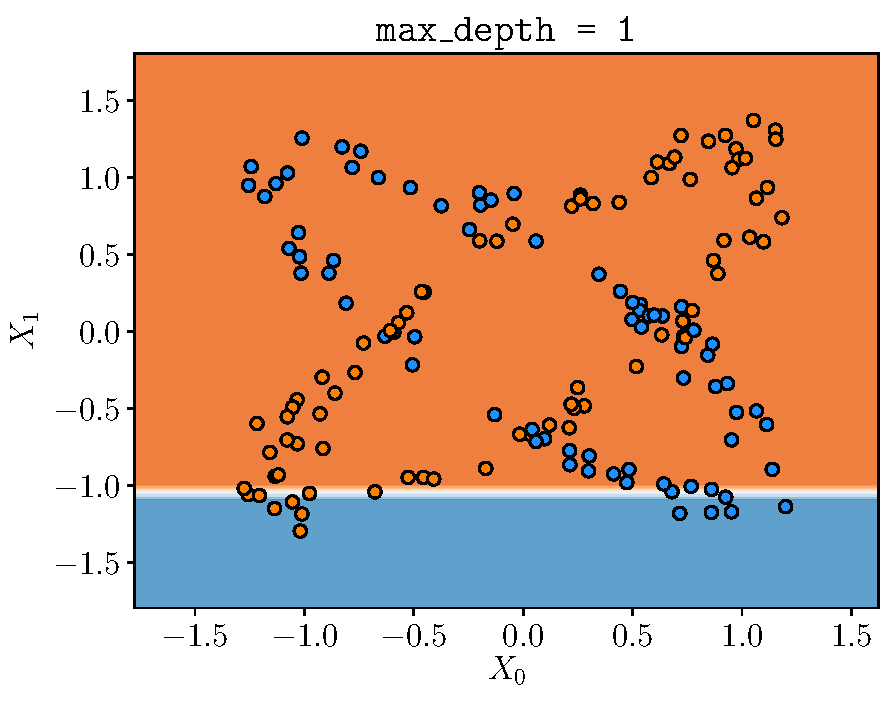
\includegraphics[width=0.85\textwidth]{resources/pdf/make_data2_depth1.pdf}
            \end{subfigure}
            \begin{subfigure}{0.49\textwidth}
                \centering
        	    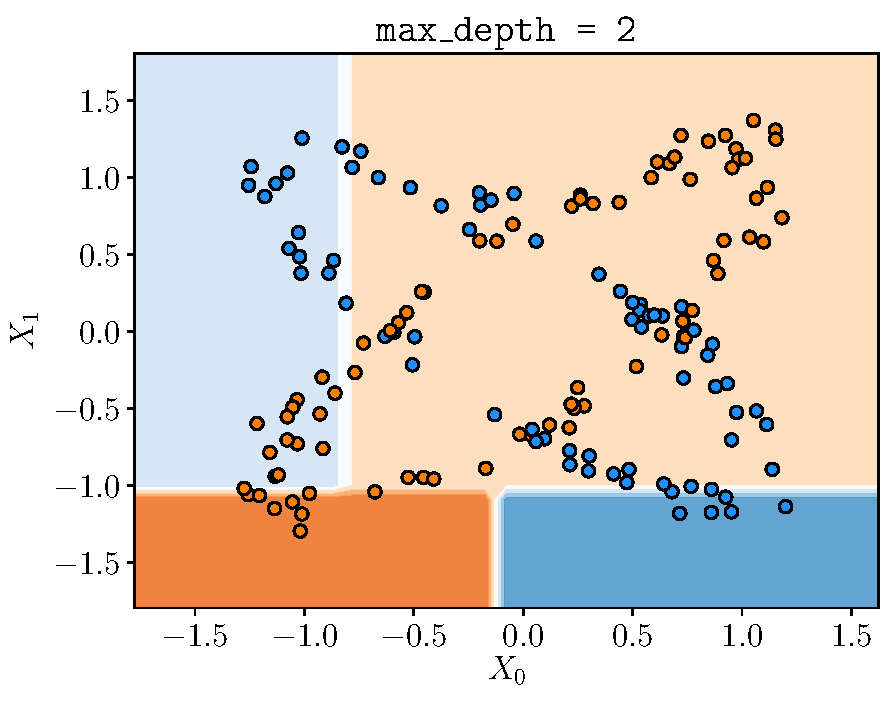
\includegraphics[width=0.85\textwidth]{resources/pdf/make_data2_depth2.pdf}
            \end{subfigure}
            \begin{subfigure}{0.49\textwidth}
                \centering
        	    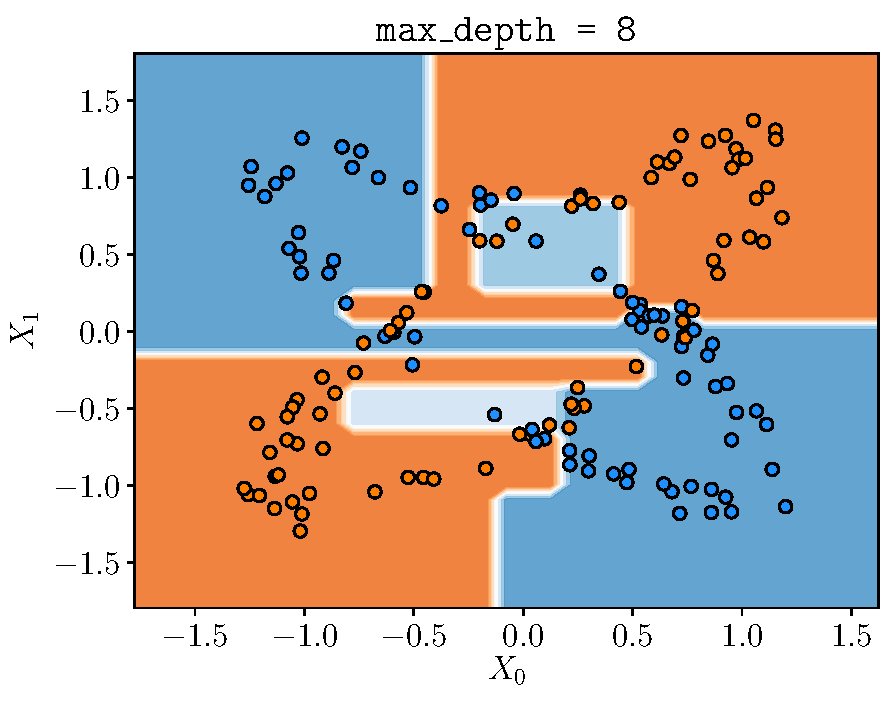
\includegraphics[width=0.85\textwidth]{resources/pdf/make_data2_depth8.pdf}
            \end{subfigure}
            \begin{subfigure}{0.49\textwidth}
                \centering
        	    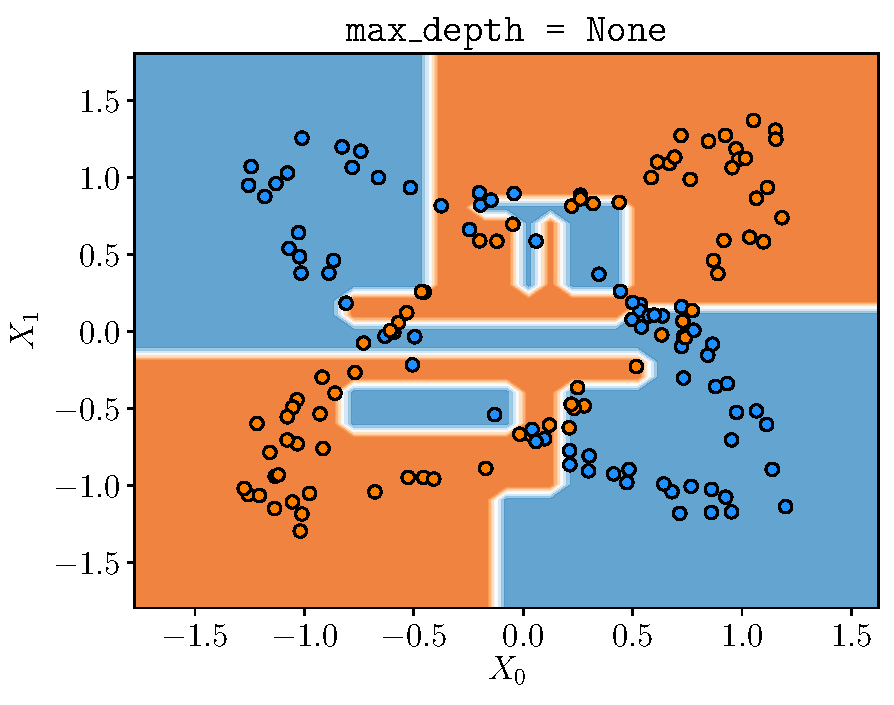
\includegraphics[width=0.85\textwidth]{resources/pdf/make_data2_depthNone.pdf}
            \end{subfigure}
            \noskipcaption{Decision boundary plots of decision tree models with fixed \texttt{max\_depth} for dataset \texttt{make\_data2}.}
            \label{fig:decision_boundary_decision_tree_make_data2}
        \end{figure}
        
        As one can see in these Figures, as the maximum depth grows, the number and complexity of boundaries do as well. Nothing surprising since the number of leafs in a decision tree is (up to) exponentially proportional to its depth.
        
        However, in the case of \texttt{make\_data1}, a complexity rise between the decision tree with a maximum depth of \num{8} and the unconstrained one isn't observable. In fact, using the \texttt{get\_depth} method of the \texttt{DecisionTreeClassifier} object, it can be shown that these two trees have the exact same depth, which means that \num{8} is a sufficient depth to classify \emph{perfectly} the \texttt{make\_data1} training set.
        
        As far as the confidence is concerned, the classifiers over \texttt{make\_data1} seem to do better than the ones over \texttt{make\_data2}, especially with low depths. Further discussion in section \ref{sec:difference}.
        
        \item For both datasets, the decision trees with maximum depth of \num{1} and \num{2} seem to underfit since the boundaries are too simple to account for the data. With a maximum depth of \num{8}, the regions begin to specialize too much, yet not enough dramaticaly  to state it is overfitting, conversely to the unconstrainded decision tree for \texttt{make\_data2} which is, indeed, overfitting.
        
        \item Unconstrained, the fitting algorithm won't stop growing the tree until it perfectly classifies the training set. At that point, each region is \emph{pure} and the model predicts the proportion of training objects of each class in the region, i.e. inevitably $1$ and $0$.
    \end{enumerate}
        %% TODO %%
        
    \subsection{Testing set accuracies} In order to compare the reliability of each model, the average testing set accuracies over five datasets generations were computed. The results are shown in Table \ref{tab:accuracies_decision_tree}.
    
    \begin{table}[h]
        \centering
        \begin{tabular}{|l|c|c|c|}
            \hline 
            Dataset & Max. depth & Average accuracy & Standard deviation \\ \hline\hline
            \multirow{5}{*}{\texttt{make\_data1}} & 1 & \num{0.684000} & \num{0.005191} \\
            & 2 & \num{0.865514} & \num{0.006390} \\
            & 4 & \num{0.890703} & \num{0.017153} \\
            & 8 & \num{0.928324} & \num{0.005572} \\
            & None & \num{0.928649} & \num{0.005071} \\ \hline
            \multirow{5}{*}{\texttt{make\_data2}} & 1 & \num{0.499784} & \num{0.007119} \\
            & 2 & \num{0.653405} & \num{0.110842} \\
            & 4 & \num{0.792216} & \num{0.024847} \\
            & 8 & \num{0.856649} & \num{0.017440} \\
            & None & \num{0.862486} & \num{0.010384} \\ \hline
        \end{tabular}
        \noskipcaption{Average testing set accuracies (over five generations of the dataset) along with their standard deviations for each depth.}
        \label{tab:accuracies_decision_tree}
    \end{table}
    
    As expected, the average accuracy increases with the depth of the decision tree. However, it does not decrease for those that have been stated as overfitting. It means that the training and testing set distributions are very close. Indeed, both datasets barely are spread around the ellipses. Also, one can see that the standard deviation of the accuracy is correlated to the overall confidence of the classifier.
   
    \subsection{Differences between the two datasets}\label{sec:difference}
    
    The first, and only, difference one can observe between \texttt{make\_data1} and \texttt{make\_data2} is their spatial distribution. While the axes of \texttt{make\_data1} ellipses are aligned with $X_0$ and $X_1$ axes, none of \texttt{make\_data2} ellipses are. In fact, by looking closely, it can be established that they are the exact same dataset (with the same \emph{seed}) but rotated \SI{45}{\degree} from each other.
    
    This angle explains why decision trees classifies better the first dataset than the second (cf. Figures \ref{fig:decision_boundary_decision_tree_make_data1}, \ref{fig:decision_boundary_decision_tree_make_data2} and Table \ref{tab:accuracies_decision_tree}), since they partition the space with axis-aligned cuts.
    
	\section{K-nearest neighbors}
	\subsection{Decision boundary}
    \begin{enumerate}[label = (\alph*)]    
        \item For both datasets (\texttt{make\_data1} and \texttt{make\_data2}) and for each \texttt{n\_neighbors} values, a decision boundary graph has been produced using the \texttt{plot\_boundary} function, yielding Figures \ref{fig:decision_boundary_neighbor_make_data1} and \ref{fig:decision_boundary_neighbor_make_data2}.
        \begin{figure}[h]
            \centering
            \begin{subfigure}{0.49\textwidth}
                \centering
        	    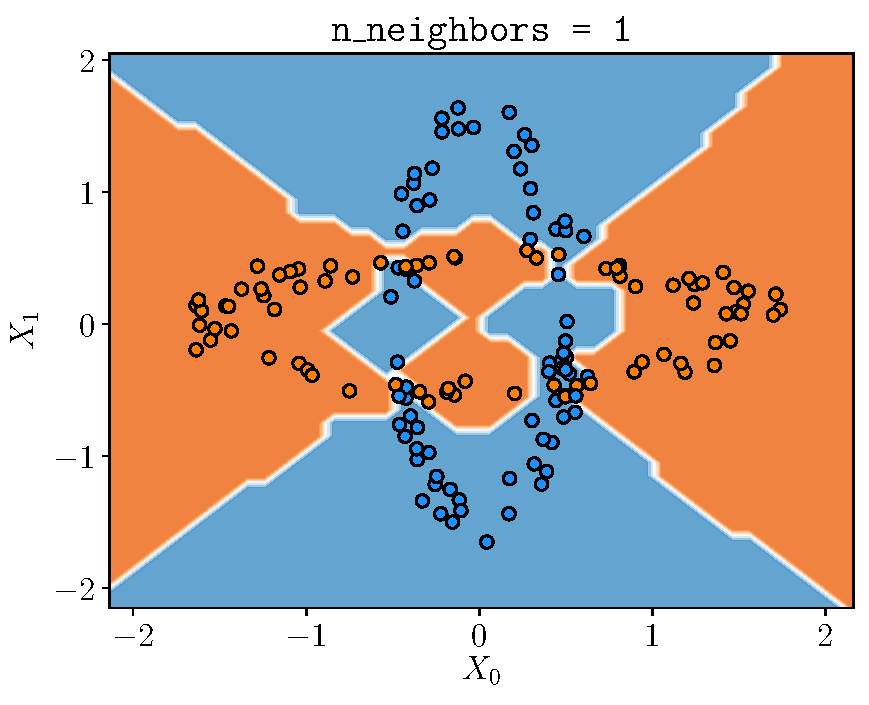
\includegraphics[width=0.85\textwidth]{resources/pdf/make_data1_neighbors1.pdf}
            \end{subfigure}
            \begin{subfigure}{0.49\textwidth}
                \centering
        	    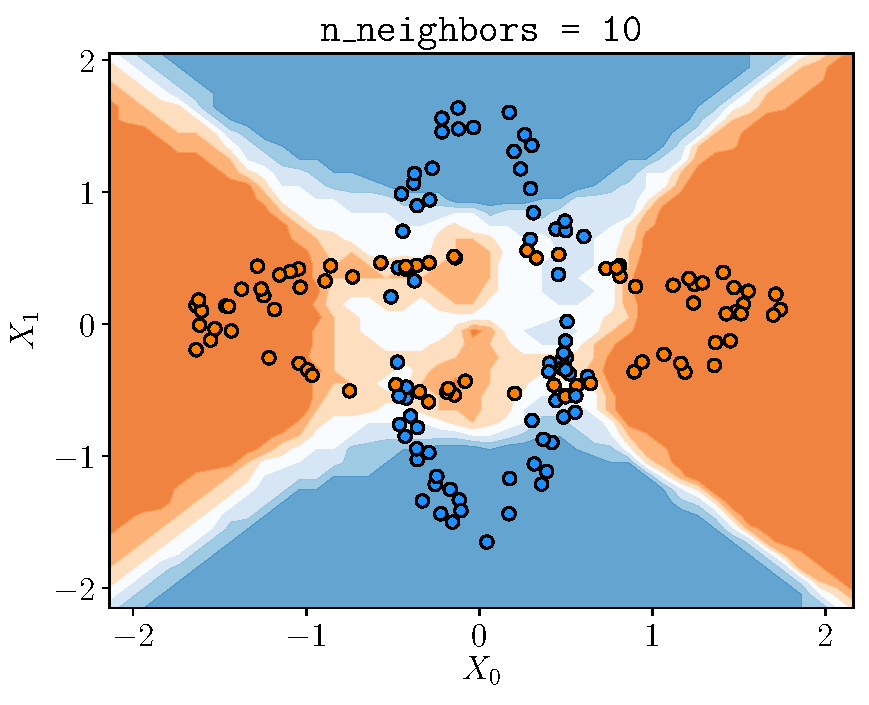
\includegraphics[width=0.85\textwidth]{resources/pdf/make_data1_neighbors10.pdf}
            \end{subfigure}
            \begin{subfigure}{0.49\textwidth}
                \centering
        	    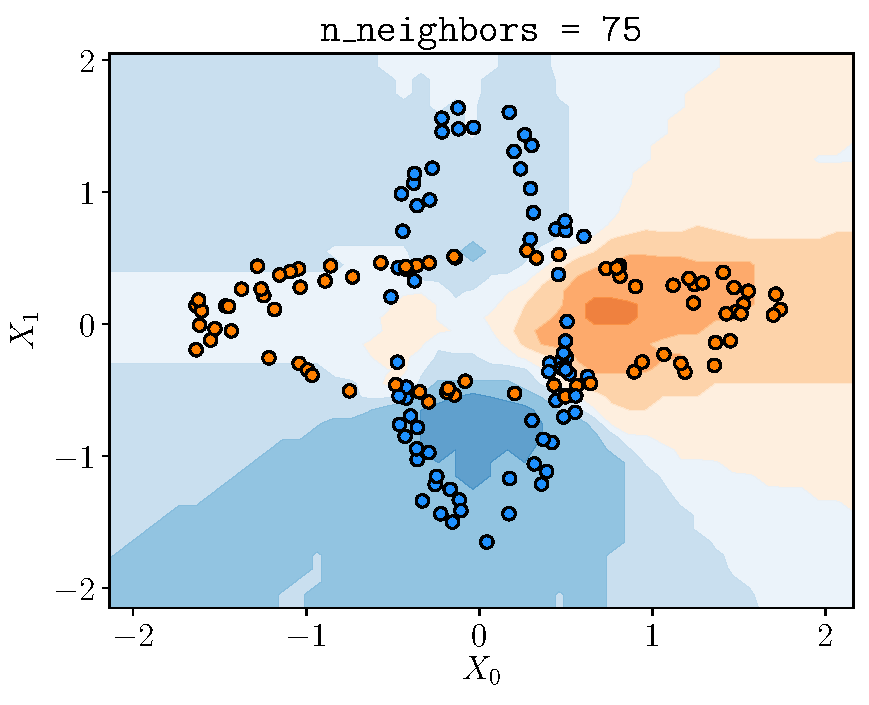
\includegraphics[width=0.85\textwidth]{resources/pdf/make_data1_neighbors75.pdf}
            \end{subfigure}
            \begin{subfigure}{0.49\textwidth}
                \centering
        	    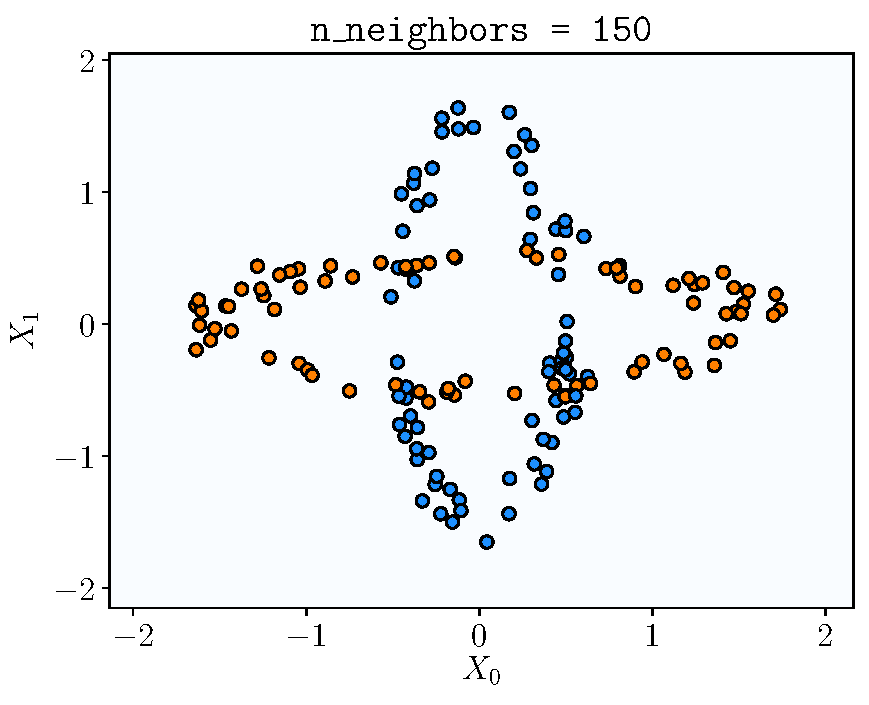
\includegraphics[width=0.85\textwidth]{resources/pdf/make_data1_neighbors150.pdf}
            \end{subfigure}
            \noskipcaption{Decision boundary plots of nearest neighbors models with fixed \texttt{n\_neighbors} for dataset \texttt{make\_data1}.}
            \label{fig:decision_boundary_neighbor_make_data1}
        \end{figure}
        \begin{figure}[h]
            \centering
            \begin{subfigure}{0.49\textwidth}
                \centering
        	    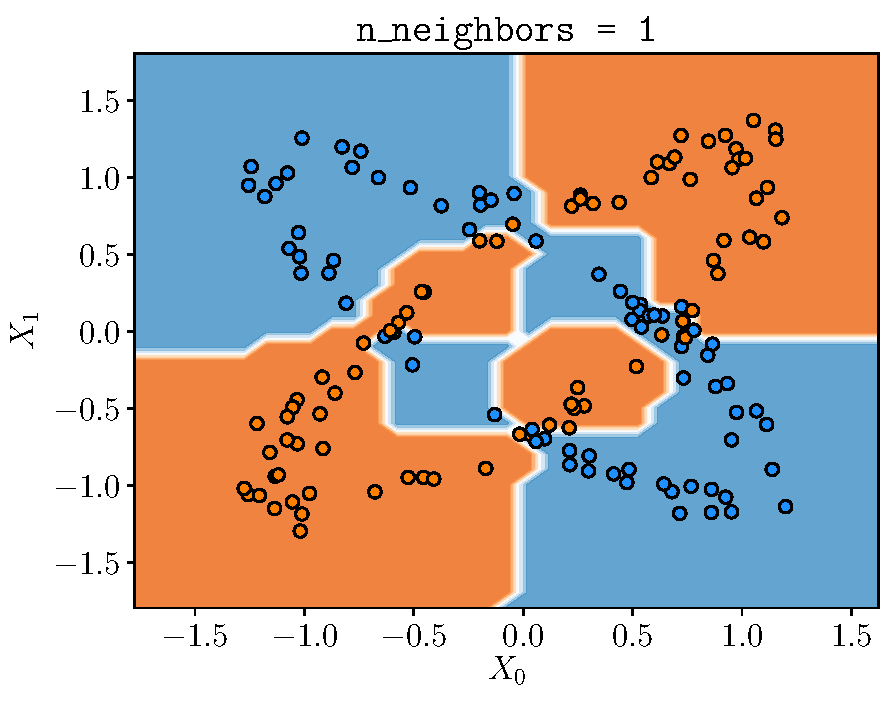
\includegraphics[width=0.85\textwidth]{resources/pdf/make_data2_neighbors1.pdf}
            \end{subfigure}
            \begin{subfigure}{0.49\textwidth}
                \centering
        	    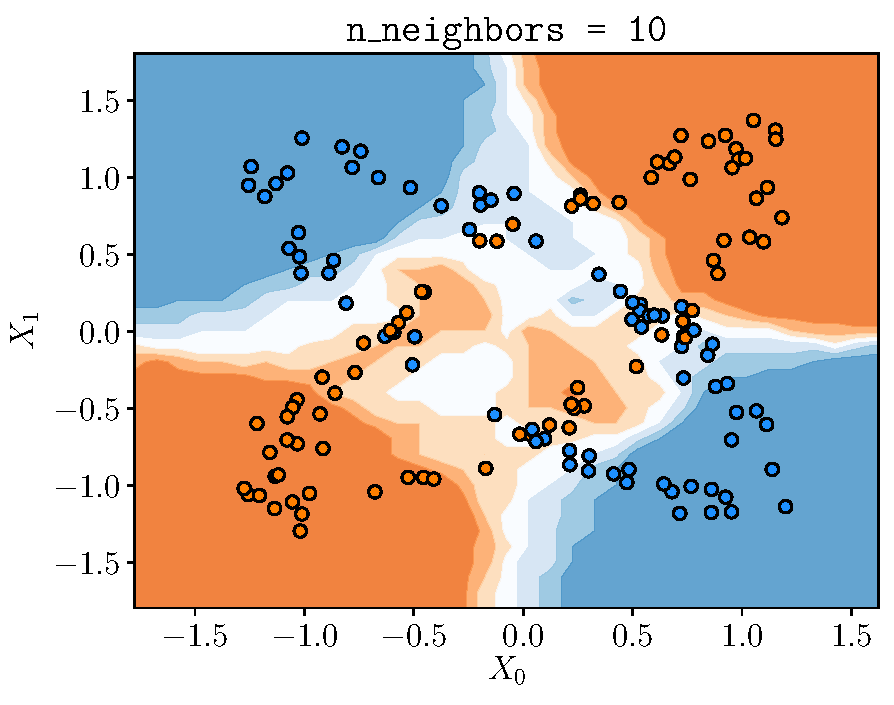
\includegraphics[width=0.85\textwidth]{resources/pdf/make_data2_neighbors10.pdf}
            \end{subfigure}
            \begin{subfigure}{0.49\textwidth}
                \centering
        	    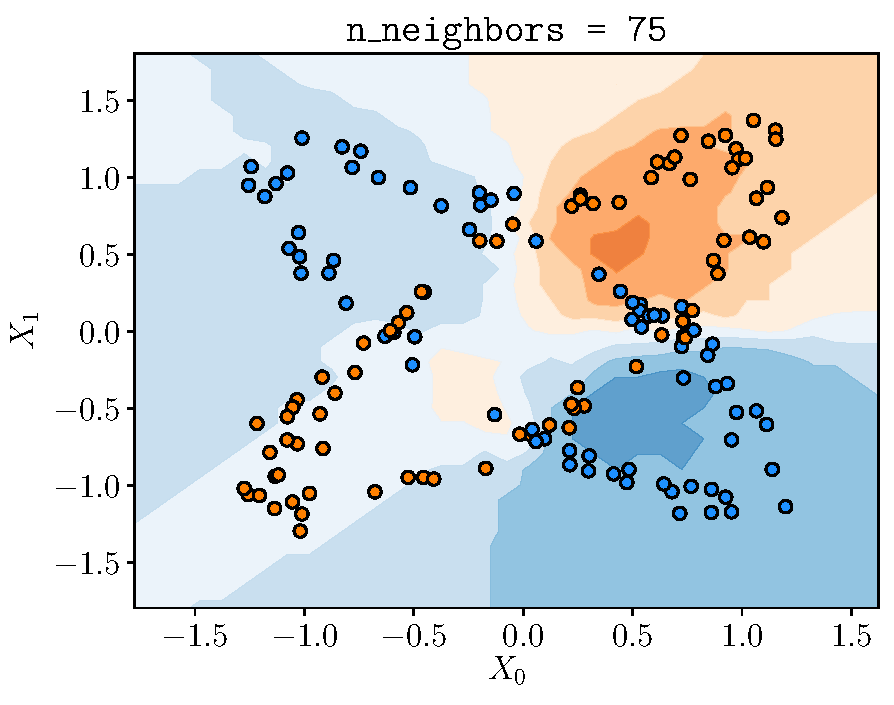
\includegraphics[width=0.85\textwidth]{resources/pdf/make_data2_neighbors75.pdf}
            \end{subfigure}
            \begin{subfigure}{0.49\textwidth}
                \centering
        	    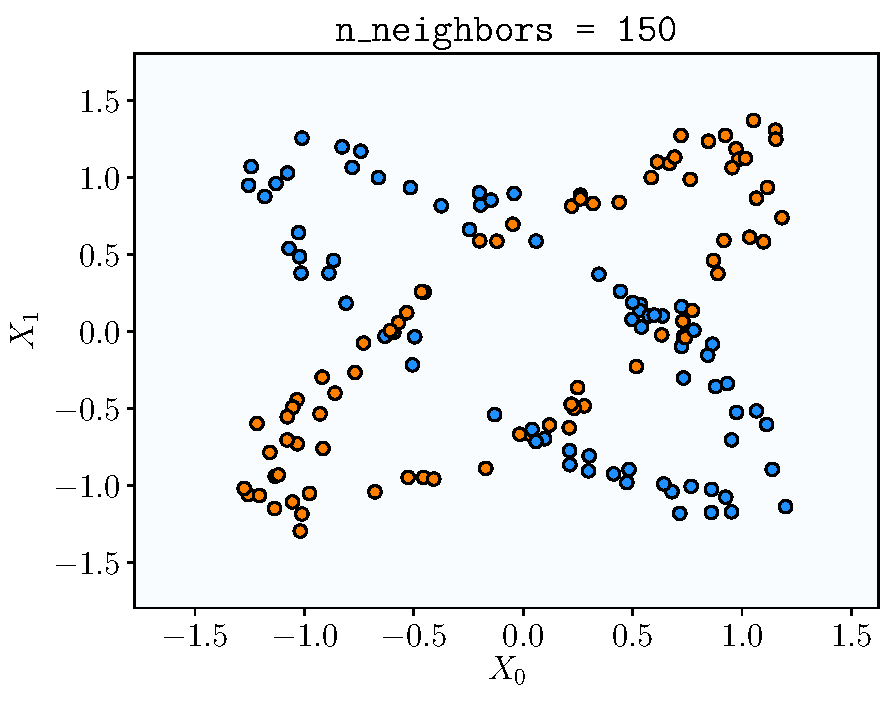
\includegraphics[width=0.85\textwidth]{resources/pdf/make_data2_neighbors150.pdf}
            \end{subfigure}
            \noskipcaption{Decision boundary plots of nearest neighbors models with fixed \texttt{n\_neighbors} for dataset \texttt{make\_data2}.}
            \label{fig:decision_boundary_neighbor_make_data2}
        \end{figure}

        \item As one can see in Figures \ref{fig:decision_boundary_neighbor_make_data1} and \ref{fig:decision_boundary_neighbor_make_data2}, as \texttt{n\_neighbors} grows, the boundaries are getting less and less sharp and the classifier confidence drops. Indeed, for \texttt{n\_neighbors = 1}, the model is \SI{100}{\percent} confident about its prediction (since it only takes the closest neighbor into account). For example, in the \emph{crossing} regions of the two ellipses, the model is still arbitrary confident, which could be depicted as overfitting.
        
        For slightly higher \texttt{n\_neighbors} values (10 to 20), the model loses its confidence in crossing regions while keeping confidence everywhere else. This is actually how the model should perform and, therefore, it is probably the most accurate.
        
        Conversely, for much higher \texttt{n\_neighbors} (40 and above), the model underfits clearly : it gives wrong predictions for most of the testing and training set objects and is poorly confident.
        
        Eventually, when \texttt{n\_neighbors} reaches the size of the training set, the prediction becomes spatially uniform since it always takes all the training set into account.
    \end{enumerate}
    
    \subsection{Ten-fold cross validation strategy}
    \begin{enumerate}[label = (\alph*)]
        \item In order to find the optimal value of \texttt{n\_neighbors}, a ten-fold cross validation strategy has been used. First, the dataset (\texttt{make\_data2}) has been split into \num{10} subsets. Each subset was then used as a testing set and its complement as a training set. Eventually, the average accuracy over the \num{10} subsets was computed for all \texttt{n\_neighbors} ranging from \num{1} to \num{100}, yielding Figure \ref{fig:ten_fold_average_accuracy}. It wasn't useful to try greater values since the average accuracy decreases for such values.
        
        \begin{figure}[h]
            \centering
            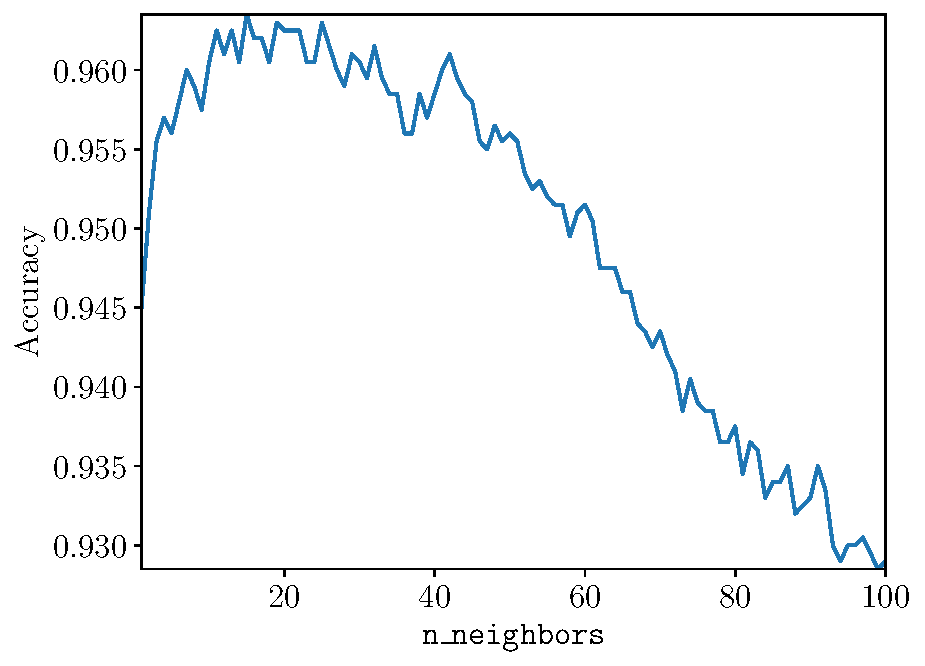
\includegraphics[width=0.6\textwidth]{resources/pdf/make_data2_kfold.pdf}
            \caption{Ten-fold cross validation average accuracy with respect to \texttt{n\_neighbors} for dataset \texttt{make\_data2}.}
            \label{fig:ten_fold_average_accuracy}
        \end{figure}
        
        \item The optimal value for \texttt{n\_neighbors} is 15 with an average accuracy of \num{0.9635}. This result corroborate the decision boundary based intuition : a good model needs to take a sufficient amount of neighbors into account in order to be less confident in crossing regions, yet not too much such that it remains confident in \emph{pure} regions.
    \end{enumerate}
    
    \subsection{Optimal value for \texttt{make\_data1}}
    Because \texttt{make\_data1} and \texttt{make\_data2} are the same datasets expressed in different (rotated) euclidean spaces (cf. section \ref{sec:difference}), the Euclidean distance between objects is conserved from one to the other. Therefore, since the k-nearest neighbors classifier is only based on that distance, the result of the ten-fold cross validation strategy should be exactly the same, that is 15. Indeed, as one can see by comparing Figures \ref{fig:decision_boundary_neighbor_make_data1} and \ref{fig:decision_boundary_neighbor_make_data2}, the decision boundary is always the same, yet rotated, for both datasets.
    
    \section{Naive Bayes classifier}
    \subsection{Equivalence}
    Let the posterior probability be $P(\Y | \X_1, \ldots, \X_p)$. Using the conditional probability definition,
    \begin{align*}
        P(\X_1, \ldots, \X_p) \, P(\Y \mid \X_1, \ldots, \X_p) & = P(\Y) \, P(\X_1, \ldots, \X_p \mid \Y) \\
        & = P(\Y) \, P(\X_1, \ldots, \X_{p - 1} \mid \Y, \X_p) \, P(\X_p \mid \Y) \\
        & = P(\Y) \, \prod_{i = 1}^{p} P(\X_i \mid \Y, \X_p, \ldots, \X_{i + 1}) \,.
    \end{align*}
    But, under the NB independence assumption,
    \begin{equation*}
        P(\X_i \mid \Y, \X_j) = Pr(\X_i \mid \Y) \quad \forall \, i, j \in \{1, \ldots, p\} \text{ and } i \neq j
    \end{equation*}
    and therefore
    \begin{align*}
        && P(\Y \mid \X_1, \ldots, \X_p) \, P(\X_1, \ldots, \X_p) & = P(\Y) \, \prod_{i = 1}^{p} P(\X_i \mid \Y, \X_p, \ldots, \X_{i + 1}) \\
        && & = P(\Y) \, \prod_{i = 1}^{p} P(\X_i \mid \Y) \, .
    \end{align*}
    And, because $P(\X_1, \ldots, \X_p)$ is independent of $\Y$, it doesn't account in \og{}$\argmax_y$\fg{} which, with the above relation, proves the equivalence between (1) and (3) in the project statement.
    
    \setcounter{subsection}{2}
    
    \subsection{Testing set accuracy on both datasets}
    The testing set accuracies on both datasets are shown in Table \ref{tab:accuracies_NB}. One can see that the Naive Bayes classifier has a better accuracy with the first dataset\footnotemark.
    
    \footnotetext{In fact, the classifier accuracy on the second dataset is near \SI{50}{\percent}, that is the accuracy a totally random classifier would obtain.}
    
    \begin{table}[h]
        \centering
        \begin{tabular}{|l|c|} \hline
            Dataset & Accuracy \\ \hline \hline
            \texttt{make\_data1} & \num{0.797838} \\ \hline
            \texttt{make\_data2} & \num{0.553514} \\ \hline
        \end{tabular}
        \noskipcaption{Testing set accuracy of both datasets using NB estimator.}
        \label{tab:accuracies_NB}
    \end{table}
    
    Actually, this is due to the NB independence assumption : the corollary to this assumption is that, knowing the class $\Y$, the correlation of every pair $\X_i, \X_j$ ($i \neq j$) is zero which is clearly misleading for \texttt{make\_data2} (cf. Table \ref{tab:correlations}) and, therefore, produces a poor model.
    
    \begin{table}[h]
        \centering
        \begin{tabular}{|l|c|c|} \hline
            Dataset & $\Y$ & $\cor(\X_0, \X_1 \mid \Y)$ \\ \hline \hline
            \multirow{2}{*}{\texttt{make\_data1}} & 0 & \num{-0.021705} \\
             & 1 & \num{-0.025280} \\ \hline
            \multirow{2}{*}{\texttt{make\_data2}} & 0 & \num{0.807203} \\
             & 1 & \num{-0.801947} \\ \hline
        \end{tabular}
        \noskipcaption{Conditional correlations of $\X_0$ and $\X_1$ in both datasets.}
        \label{tab:correlations}
    \end{table}
\end{document}
